\begin{minipage}{0.5\textwidth}
    In this assignment, 
    you will use \myEmph{linear regression} to find the 
    {\itshape line of best fit} using both 
    \myDesmos and a \myTi calculator.
    
    Here are the data you will use.
\end{minipage}
\begin{minipage}{0.29\textwidth}
\begin{center}
    \large
    \begin{tabular}{cc}
        \toprule 
        $x$ & $y$ \\ 
        \midrule
        0.00 & -3.00 \\
        2.00 & 14.96 \\
        4.00 & 19.94 \\
        6.00 & 10.12 \\
        8.00 & 55.06 \\
        10.00 & 64.70 \\
        12.00 & 50.5 \\ 
        13.00 & 70 \\
        \bottomrule
    \end{tabular}
\end{center}
\end{minipage}

\myWideProblemWithContent
{
    Sketch a scatterplot for the data in the table.\newline
    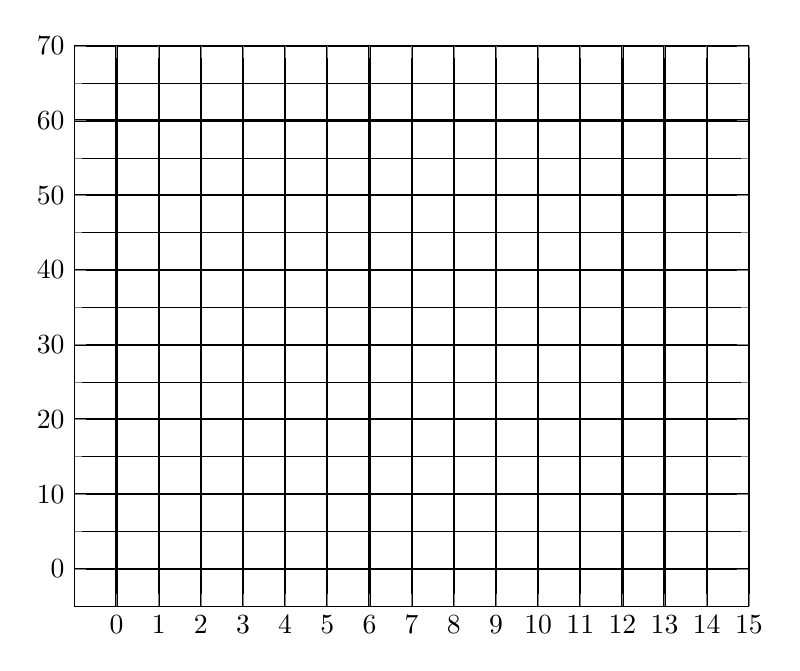
\begin{tikzpicture}
        \begin{axis}[
            scale=1.25,
            grid = both,
            xmin=-1, xmax=15, xtick distance=1, xtickmin=0,
            ymin=-5, ymax=70, ytick distance=10, minor y tick num=1,
            major grid style={solid,thick,black},
            minor grid style={solid,very thin,black},
        ]
        \end{axis}
    \end{tikzpicture}
}